\chapter[Electron Charge Asymmetry]{ 
Measurement of the electron charge asymmetry with \unit{36}{\invpb} }

In this chapter the first measurement of the electron charge asymmetry in
inclusive \inclusiveWe production with the \ac{CMS} detector is described.

The analysis is performed on the full 2010 dataset, which corresponds to a
luminosity of \unit{36.1}{\invpb}.

\section{Event Selection}

The event selection used in this analysis is based on a limited number of cuts.
This is due to the limited statistics available in early data taking.

\subsection{Trigger}

\label{asym36:triggerdef}
Several triggers were used to select the events, due to the increasing
luminosity in the \ac{LHC} 2010 run.

In the initial runs, events were selected using only a single photon trigger. 
As the luminosity increased these triggers became prescaled it was
necessary to use electron triggers to select events. 
As the luminosity increased even further, it was necesary to use electron
triggers that included cuts on electron ID variables.

The triggers used to select the events are sumarised in \TableRef{asym36:triggers}
where HLT\_Ele$X$ indicates a selection requiring a $\Pt > \unit{X}{\GeV}$. 
``Photon'' in the name indicates that the selection was applied to ECAL
superclusters rather than an electron. 
``SW'' stands for small window, where window refers to the electron
pixel-matching window. 
 ``Cleaned'' indicates that spikes in the \ac{ECAL} have been removed. 
``CaloEleId'' and ``TightCaloIdIso'' represent increasingly tighter selection
based on ID variables from only the \ac{ECAL}.  This is done to allow us to
obtain a control sample by inverting other ID variables.
``TightCaloIdIso'' indicates a tight selection based on all ID variables. 
This was the only trigger available for these runs, a looser prescaled
selection has also been applied in these runs for the control sample.

\begin{table}[htb]
  \centering
  \begin{tabular}{ l l }
    Run Ranges & Trigger \\
    \midrule
    132440-137028 & \verb=HLT_Photon10_L1R= \\
    138564-140401 & \verb=HLT_Photon15_Cleaned_L1R= \\
    141956-144114 & \verb=HLT_Ele15_SW_CaloEleId_L1R= \\
    146428-147116 & \verb=HLT_Ele17_SW_CaloEleId_L1R= \\
    147196-148102 & \verb=HLT_Ele17_SW_TightEleId_L1R= \\
                  & \verb=HLT_Ele17_SW_L1R (prescaled)= \\ 
    148822-149063 & \verb=HLT_Ele22_SW_TighterCaloIdIso1_L1R_v1= \\
    149181-149442 & \verb=HLT_Ele22_SW_TighterCaloIdIso1_L1R_v2= \\
  \end{tabular}
  \caption{Triggers used to select the data used in this analysis.}
  \label{asym36:triggers}
\end{table}

\subsection{Electron Selection}

The available unprescaled triggers constrain the electron momentum to be above
\unit{25}{\GeV}.

Electrons candidates are identified using a cut based approach on an limited
number of variables.

The cuts can be split in to three categories, ID Cuts, isolation cuts and
conversion rejection cuts. Different sets of cut values are used for electrons in the
ECAL barrel and endcap. The cut values are obtained by simultaneous optimisation
for electron \unit{\ET=25}{\GeV}. Although the efficiency and and the background
rejection of the cuts is dependent on the \ET of the electron, the cut values
obtained are found to be effective in the range \unit{15-100}{\GeV}.\cite{}

\TableRef{tab:elecuts} sumarises the electron selection variables used and the
corresponding cut values for the barrel and endcap.

\todo{tie this in with physics objects chapter}

%% TODO finish ZZZzzzzz,,,,
\begin{table}[htbp]
  \begin{center}
    \leavevmode
    \begin{tabular}{lcc} 
      \multicolumn{1}{c}{Variable} & \multicolumn{1}{c}{cut value (barrel)}& \multicolumn{1}{c}{cut value (endcap)}\\
      \hline
      \multicolumn{3}{l}{ID Cuts}\\ 
        H/E & 0.04 & 0.025 \\
        $\Delta\phi$ & 0.06 & 0.03 \\
        $\Delta\eta$ & 0.004 & 0.007  \\
        $\sigma_{\eta\eta}$ & 0.01 & 0.03 \\ \hline
      \multicolumn{3}{l}{Isolation Cuts}\\
        $ISO_{trk} / E_T $  & 0.09 & 0.04 \\
        $ISO_{ecal}/ E_T$  & 0.07 & 0.05 \\
        $ISO_{hcal}/ E_T$  & 0.10 & 0.025 \\ \hline
       \multicolumn{3}{l}{Conversion Rejection Cuts}\\ 
        Missing Hits  & \multicolumn{2}{c|}{$\leq 0$}\\
        Dist $||$ Dcot   & \multicolumn{2}{c|}{$>0.02$}\\
    \end{tabular}
    \caption{\label{tab:elecuts} Electron selection variables and corresponding cut values.}
  \end{center}
\end{table}


Mismeasuring the charge can lead to a diltuion of the measured charge asymmetry,
to overcome this an additional requirement is applied to the charge of the
reconstructed electron. 
The electron charge is determined using three different methods based on the GSF
electron charge, the general track charge and the supercluster charge.

The charge mismeasurment can be measured at the Z peak by comparing the same
sign \HepProcess{\PZ\to\Pepm\Pepm} yield to the oposite sign
\HepProcess{\PZ\to\Pepm\Pemp} yield. \FigureRef{fig:charge} show these Z yields
using only the \ac{GSF} track charge (black) and also requiring a unaminous
asignment of charge from all three methods (red). 


The charge mismeasurement rate from the GSF track charge is about \unit{3}{\%}.
By requiring that all three methods for assigning the charge agree, and vetoing
events otherwise, the mismeasurement can be reduced by a factor of 8 with only a
\unit{5}{\%} loss in efficiency.

\begin{figure}[htb]
  \begin{center}
\includegraphics*[height=0.4\textwidth, angle=90]{Zchargeall.pdf}
\includegraphics*[height=0.4\textwidth, angle=90]{ZchargeSS.pdf}
 \caption{ \label{fig:charge} $Z\rightarrow ee$ peak. One electron is required to be in the barrel to pass the VBTF80 selection
  and to have a fraction of energy loss by radiation less than 0.3; the second electron is required only to pass the VBTF80 selection. Left: all combinations. Right: Same sign combinations.}
  \end{center}
\end{figure}

                     

\subsection{Event Selection}

An Event is selected if if contains a single electron that passes all electron
selection.
To removed Drell-Yan events an event is vetoed if it contains a second lepton
(an electron passing a loose selecton, or an isolated muon) with $\PT > 
\unit{15}{\GeV}$

The Particle Flow \ETm distribution for the events that pass the event
selection, with $\PT > \unit{25}{\GeV}$ and $|\eta| < 2.4$ is shown in
\FigureRef{asym36:pfmet}.
The number of selected events that pass the event selection are shown in
\TableRef{asym36:selectedevents}.



\begin{figure}[htb]
  \begin{center}
    \includegraphics*[width=0.45\textwidth]{h_pfmet_nostat}
    \caption{Particle Flow transverse missing energy (PFMET) distribution for selected events.}
  \label{asym36:pfmet}
  \end{center}
\end{figure}


\begin{table}[htb]
\begin{center}
\begin{tabular}{lcrrrr}
  $|\eta|$ range & Charge & \multicolumn{4}{c|}{Selected Events}\\
                 &        & $\PT>25$ \GeV & $\PT>30$ \GeV & $\PT>35$ \GeV  & $\PT>25$ \GeV  \\
                 &        &               &               &                & $\ETm>20$ \GeV \\
\hline
$0.0<| \eta |<0.4$ &+& 18956&14232&9885&14213\\
                   &-& 15060&11505&8105&10587\\
$0.4<| \eta |<0.8$ &+& 20118&14966&10345&14702\\
                   &-& 15736&11780&8307&10734\\
$0.8<| \eta |<1.2$ &+& 20681&15091&10184&14231\\
                   &-& 16167&11735&8112&10247\\
$1.2<| \eta |<1.4$ &+& 10646&7606&5161&6789\\
                   &-& 8226&5871&4067&4713\\
$1.6<| \eta |<2.0$ &+& 16426&11877&7814&10827\\
                   &-& 11678&8578&5886&6802\\
$2.0<| \eta |<2.4$ &+& 18885&13239&8726&10991\\
                   &-& 13226&9227&6184&6439\\
\end{tabular}
\caption{Number of events passing the event selection for lepton momentum cut of $\PT>25$ \GeV, $\PT>30$ \GeV and $\PT>35$ \GeV .}
    \label{asym36:selectedevents}
\end{center}
\end{table}
% TODO REMOVE MET CUT
\todo{remove met cut from tables}


The exected composition of the selected events, derived from MC simulation
samples, is show in \TableRef{asym36:selectedcomp}. 

\begin{table}[htb]
\begin{center}
\begin{tabular}{lrrrr}
& $\PT>25$ \GeV & $\PT>30$ \GeV & $\PT>35$ \GeV  & $\PT>25$ \GeV  \\
&  & &  &  $\ETm>20$ \GeV \\ \hline
$W\rightarrow e\nu$  & $65.1\%$&$63.5\%$ &$60.2\%$  &$95.3\%$\\
QCD Background       & $28.2\%$&$31.3\%$ &$35.7\%$  &$1.5\%$\\
EWK Total Background & $6.7\%$ &$5.2\%$  &$4.1\%$   &$3.2\%$ \\
~ EWK DYtautau         & $0.4\%$ &$0.3\%$  &$0.2\%$   &$0.2\%$ \\
~ EWK DYee             & $4.1\%$ &$3.5\%$  &$3.0\%$   &$0.3\%$ \\
~ EWK Wtaunu           & $1.9\%$ &$1.1\%$  &$0.6\%$   &$2.3\%$ \\
~ EWK ttbar            & $0.3\%$ &$0.3\%$  &$0.3\%$   &$0.4\%$ \\
\end{tabular}
\caption{Composition of selected events for lepton momentum cut of $\PT>25$ \GeV, $\PT>30$ \GeV and $\PT>35$ \GeV .}
\label{asym36:selectedcomp}
\end{center}
\end{table}


\section{Signal Yield Extraction}

The number of signal and background events in each bin is extracted using a fit
to the \ETm distribution using two templates.
The first is the sum of the \Wenu signal and the \ac{EWK} background shapes,
and the second is the sum of the \ac{QCD} plus \gjet processes.

\subsection{\ac{QCD} \ETm Shape}

The \ac{QCD} and \gjet background distribution is obtained from a control sample of
events. The control sample is selected by requiring that the electrons pass the
isolation and H over E cuts but fail the $\Delta\phi$ and $\Delta\eta$ cuts as
shown in \TableRef{asym36:antisel}.

\begin{figure}[htb]
  \begin{center}
    \includegraphics*[width=0.3\textwidth, angle=90]{MetCompare_anti_eta1.pdf}
    \includegraphics*[width=0.3\textwidth, angle=90]{MetCompare_anti_eta2.pdf}
    \includegraphics*[width=0.3\textwidth, angle=90]{MetCompare_anti_eta3.pdf}
    \includegraphics*[width=0.3\textwidth, angle=90]{MetCompare_anti_eta4.pdf}
    \includegraphics*[width=0.3\textwidth, angle=90]{MetCompare_anti_eta5.pdf}
    \includegraphics*[width=0.3\textwidth, angle=90]{MetCompare_anti_eta6.pdf}
    \caption{\label{fig:MetComparison} The \ETm\ distribution of anti-selected Monte Carlo simulated events and selected QCD and $\gamma +jet$ events for each eta bin.}
  \end{center}
\end{figure}

\begin{table}[htbp]
  \begin{center}
    \leavevmode
    \begin{tabular}{lcc} 
      \multicolumn{1}{c}{Variable} & \multicolumn{1}{c}{cut value (barrel)}& \multicolumn{1}{c}{cut value (endcap)}\\\hline
        H/E & 0.04 & 0.025 \\
        $\Delta\phi$ & $>0.06$  & $>0.04$ \\
        $\Delta\eta$ & $>0.007$ & $>0.009$\\
        $ISO_{trk} / E_T $ & 0.09 & 0.04 \\
        $ISO_{ecal}/ E_T$  & 0.07 & 0.05 \\
        $ISO_{hcal}/ E_T$  & 0.10 & 0.025\\ 
    \end{tabular}
    \caption{\label{tab:AScuts}Electron anti-selection variables and corresponding cut values. $\Delta\phi$ and $\Delta\eta$ cuts are inverted.}
  \end{center}
\end{table}


To validate the antiselection used, \ac{QCD} \ac{MC} samples are used. The
distribution of \ac{QCD} events passing the event selection are comapred to the
antselected MC events. This is shown for each eta bin in
\FigureRef{asym36:antiselclosure}.

\begin{figure}[htb]
  \centering
  %
\includegraphics[width=0.5\textwidth]{placeholder}
  \caption{The \ETm distribution on antiselected \ac{MC} simulated events
  and selected \ac{QCD} and \gjet events in each pseudorapidity bin.}
  \label{asym36:antiselclosure}
\end{figure}

\subsection{Signal \ETm Shape from Boson Recoil}

The Signal \ETm shape was obtained using information from the recoil of the
boson

\todo{add more information on the hoson recoil method.}

\subsection{\ac{EWK} \ETm Shape}

The \ac{EWK} background \ETm distributions were obtained from Pythia \ac{MC}
simulations.

\todo{add more information on the EWK template shape.}

\subsection{Validation of Signal Extraction Method on Simulation}

The signal yield extraction procedure was validated using pseudodata
experiments. 1000 pseudodata experiments were generated with the number of
events expected in \unit{36.1}{\invpb} of data. The signal yields are extracted
in each experiment and the asymmetry is calculated. The distribution of
asymmetries is then fitted with a gaussian.

The width of the gaussian is the statistical uncertainty on the measurement.

The statistical uncertainty can aslo be estimated from the following formula


\begin{equation}
  \label{asym36:statuncert}
   \frac{d\mathcal{A}_{stat}}{d\eta} =
   \frac{2 \times \sqrt{ 
       \left( \frac{dN^+}{d\eta} \sigma_{\frac{dN^-} {d\eta}}\right)^2 + 
       \left( \frac{dN^-}{d\eta} \sigma_{\frac{dN^+} {d\eta}}\right)^2  }}
   {\left(  \frac{dN^+}{d\eta} +  \frac{dN^-}{d\eta} \right)^{2} }
\end{equation}

The uncertainty from \EquationRef{asym36:statuncert} evaulated with \ac{MC} truth
values, and the uncertainty measured from pseudodata experiments for an
integrated luminosity of \unit{36.1}{\invpb} are summarised in
\TableRef{asym36:statuncertsum}.

\begin{table}[htb]
  \begin{center}
    \begin{tabular}{lcc}
    $|\eta|$ range & $\sigma_{A}$ from \EquationRef{asym36:statuncert}. & $\sigma_{A}$ from pseudo-data exp.\\ \hline
    $0.0<|\eta|<0.4$ & 0.0064 & 0.0062\\
    $0.4<|\eta|<0.8$ & 0.0064 & 0.0064\\
    $0.8<|\eta|<1.2$ & 0.0065 & 0.0065\\
    $1.2<|\eta|<1.4$ & 0.0096 & 0.0104\\
    $1.6<|\eta|<2.0$ & 0.0076 & 0.0079\\
    $2.0<|\eta|<2.4$ & 0.0077 & 0.0077\\
    \end{tabular}
  \caption{Expected statistical error as a function of pseudorapidity, for an
  integrated luminosity of \unit{36}{\invpb}. }
  \label{asym36:statuncertsum}
  \end{center}
\end{table}


%For each of the pseudo-data experiments we calulated the pull on the asymmetry measurement.
%The pull is defined as the diffence between the measured asymmetry for a pseudo-data experiment
%and the MC true value divided by the statistical uncertainty, and represents the number of standard deviations away from the true value.
%The distribution of the pulls from 1000 pseudo-data experiments are shown in figure \ref{fig:toyasym_pull}, and are fitted with a gaussian.
%It is expected that the mean of this gaussian is zero for an unbiased measurement and the
%sigma is one for a measurement with well understood statistical uncertainties.

\begin{figure}[htb]
  \begin{center}
    \includegraphics*[angle=90,width=0.95\textwidth]{toyasym.pdf}
    \caption{\label{fig:toyasym}Measured Asymmetry for 1000 pseudo-data experiments. The distribution of the measured Asymmetry is fitted with a gaussian.}
  \end{center}
\end{figure}

\begin{figure}[htb]
  \begin{center}
\includegraphics*[angle=90,width=0.95\textwidth]{pullasyTot.pdf}
    \caption{\label{fig:toyasym_pull}Pull on the Asymmetry in 1000 pseudo-data experiments. The distribution of the pull is fitted with a gaussian.}
  \end{center}
\end{figure}

\subsection{Fit on Real Data}


\begin{figure}
  \begin{center}
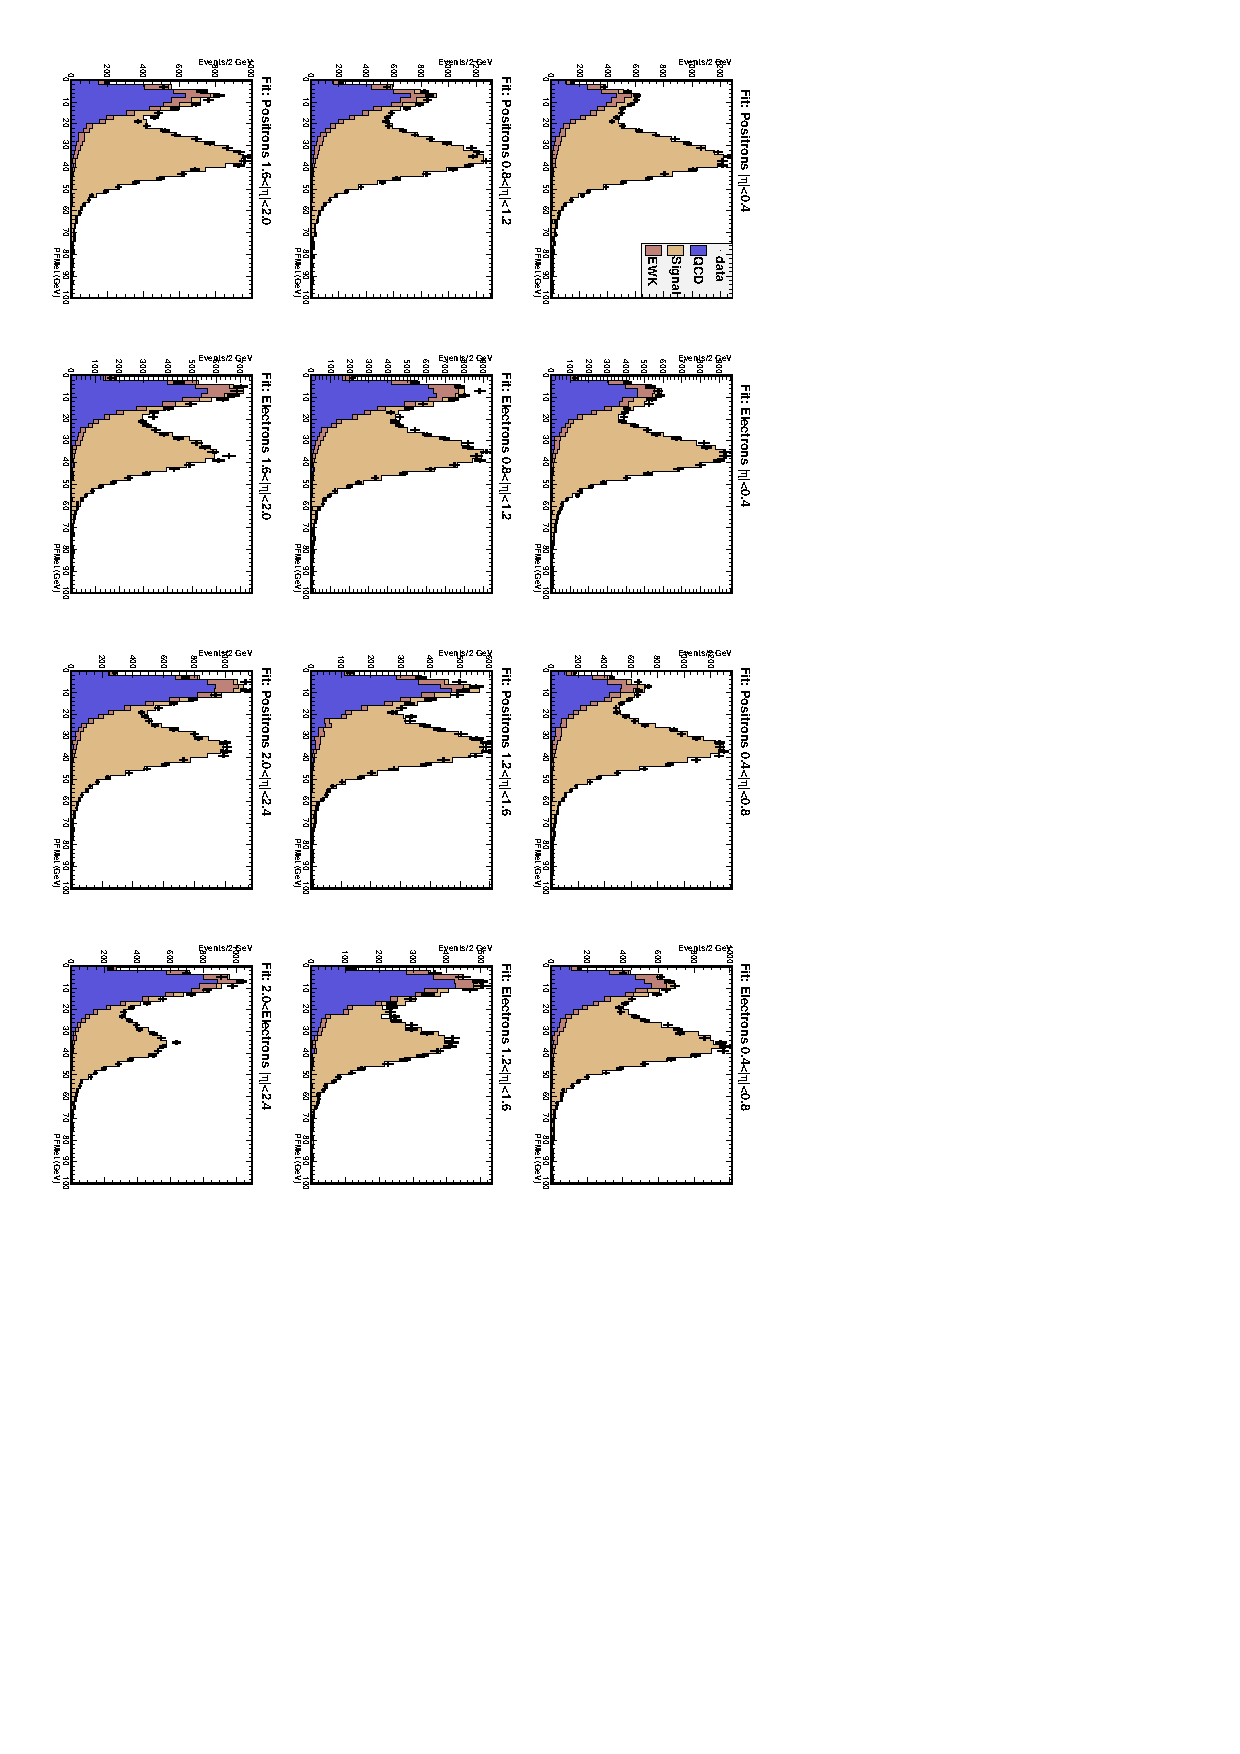
\includegraphics[angle=90,width=0.95\textwidth]{Dec22_data}
 \caption{  \label{fig:data} The fit to \ETm\ for each eta/charge bin.}
  \end{center}
\end{figure}

\begin{figure}
  \begin{center}
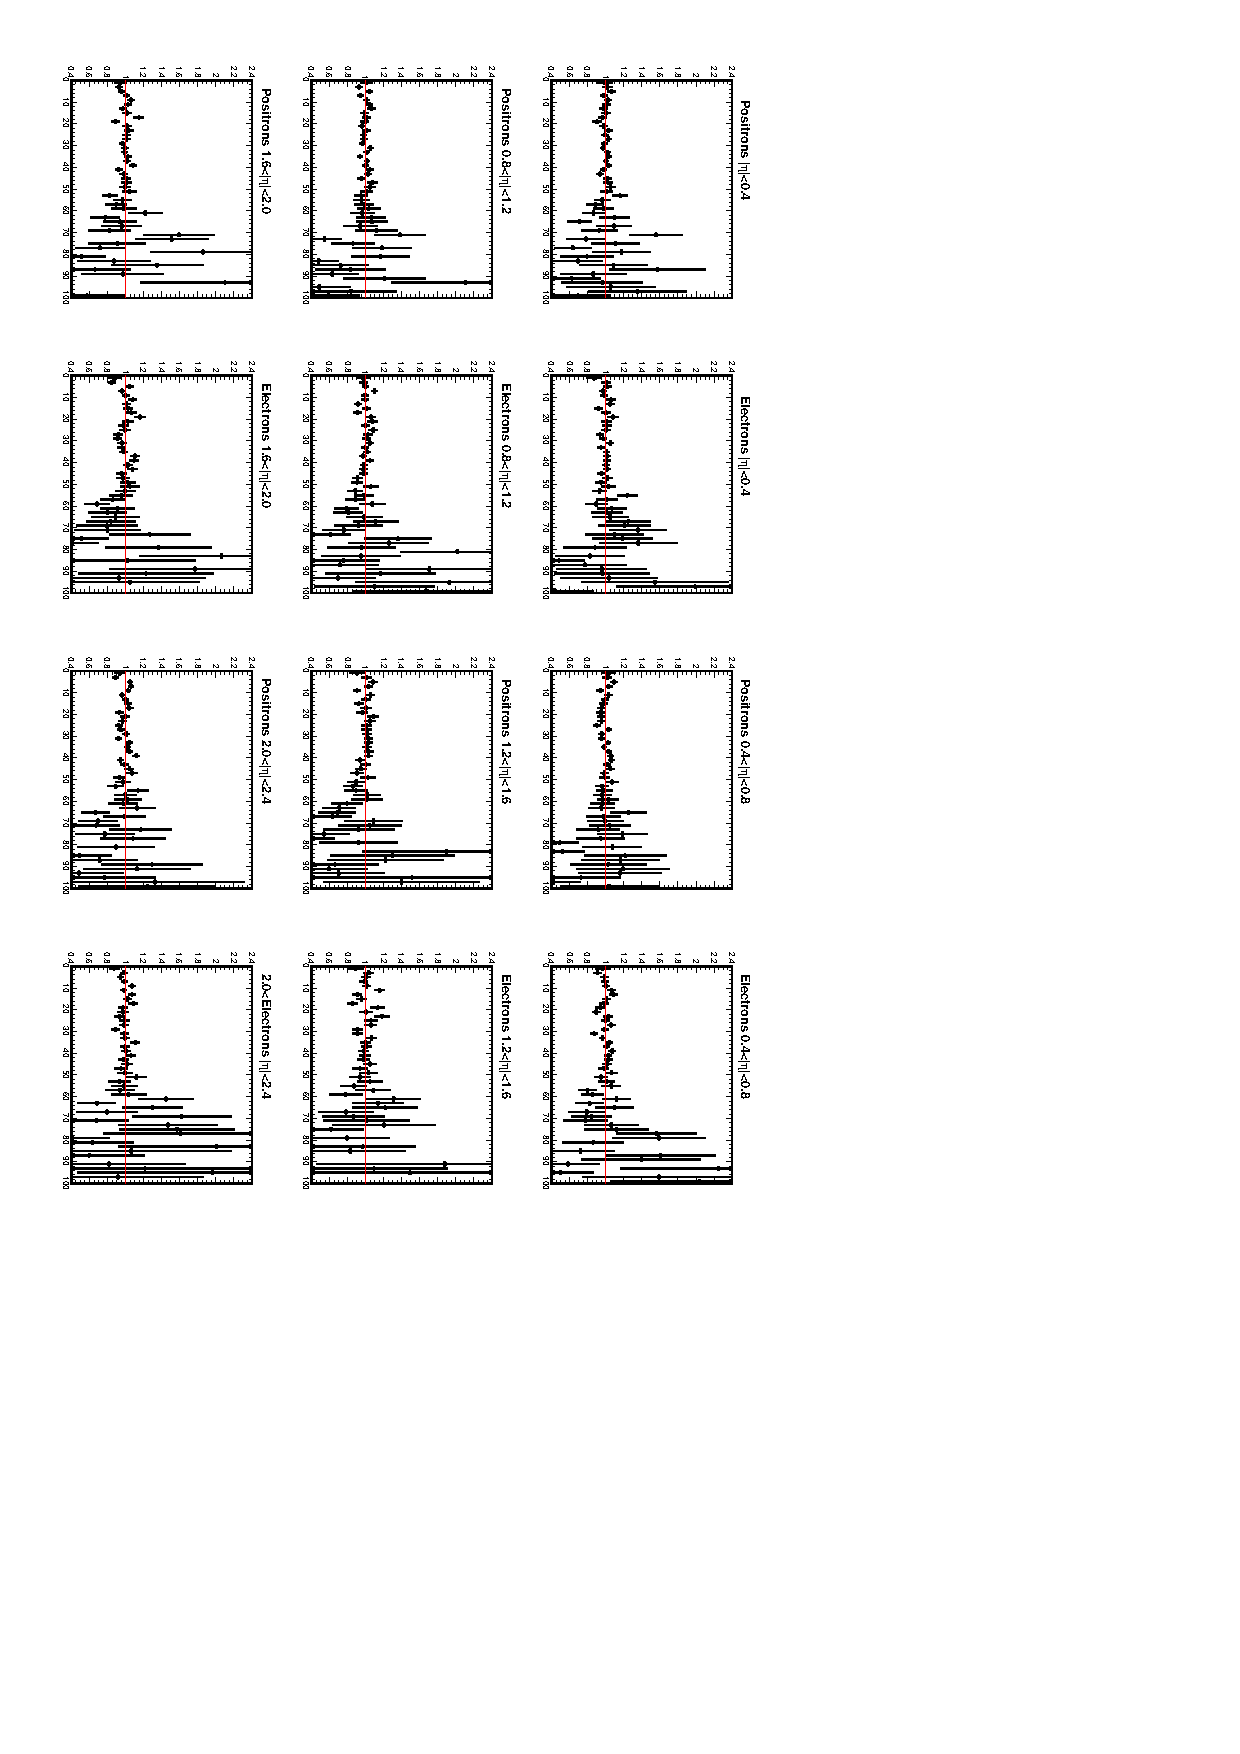
\includegraphics[angle=90,width=0.95\textwidth]{Dec22_fitratio}%width=0.9\textwidth,
     \caption{\label{fig:datafitratio}Ratio between fit and data for each eta/charge bin.}
  \end{center}
\end{figure}

\begin{table}[htb]
\begin{center}
\begin{tabular}{|lc|r|}
$|\eta|$ range &Charge & $\chi^2$/ndof of Fit\\
\hline
$0.0<| \eta |<0.4$ &+&  0.86\\
                   &-&  0.84\\
$0.4<| \eta |<0.8$ &+&  0.99\\
                   &-&  1.36\\
$0.8<| \eta |<1.2$ &+&  1.05\\
                   &-&  1.13\\
$1.2<| \eta |<1.4$ &+&  0.97\\
                   &-&  1.30\\
$1.6<| \eta |<2.0$ &+&  1.38\\
                   &-&  1.61\\
$2.0<| \eta |<2.4$ &+&  1.44\\
                   &-&  1.11\\
\end{tabular}
\caption{\label{tab:chi2}$\chi^2$/ndof of Fit.}
\end{center}
\end{table}

\section{Systematic Uncertainties}
\subsection{Relative Efficiency}

If the reconstruction efficiency of electrons is different to that of positrons
then the measured asymmetry wil be diluted and will need to be corrected for
the relative efficiency.

\begin{equation}
A_{exp}(\eta) = \frac{
                    \frac{dN}{d\eta}(e^+)-
                    \frac{\epsilon^+}{\epsilon^-}\frac{dN}{d\eta}(e^-)
                }
                {
                    \frac{dN}{d\eta}(e^+)+
                    \frac{\epsilon^+}{\epsilon^-}\frac{dN}{d\eta}(e^-)
                }
\end{equation}

The efficiency for electrons and positrons is measured using the tag and probe
method \todo{reference the CMS tag and probe method paper/note}
with a sample of \Zee events from the same datasets used in the analysis. 
The \Zee events offer a high purity source of unbiased electrons with which to
measure the efficiencies.

From the sample of \Zee events a ``tag'' electron is selected with a strict
selection criteria. 
A ``probe'' electron is selected with the same electron selection decribed
earlier.
The invariant mass of the tag-probe pair is required to be
$\unit{60}{\GeV} < M_ee < \unit{120}{\GeV}$ to ensure a high purity sample.

Efficiencies can then be calculated by measuring the signal yield in events
with one tag electron and one probe passing the selection (tag \& pass) and
events where the probe electron fails the selection (tag \& fail).
The signal yield is extracted using an simultaneous maximum likelihood fit to
both the tag \& pass and the tag \& fail samples.

For this analysis the efficiencies are measured in two parts:

\begin{itemize}
    \item GSF tracking efficiency
    \item Identification efficiency, including conversion rejection, unaminous
charge assignment and HLT request.
\end{itemize}

\begin{table}[htbp]
\begin{center}
\begin{tabular}{cccccccc}
$|\eta|$  & \multicolumn{3}{c}{GSF tracking } & \multicolumn{3}{c}{ID } & $R_\epsilon$ \\
region    & $\epsilon_{GSF}^+$ (\%) &$\epsilon_{GSF}^-$ (\%) & $R_{\epsilon_{GSF}}$ 
                                              & $\epsilon_{ID}^+$ (\%) &$\epsilon_{ID}^-$ (\%) & $R_{\epsilon_{ID}}$ &  \\
\hline
$\left[ 0.0,0.4 \right]$ & 95.7$\pm$1.1 & 97.5$\pm$1.0 & 0.982$\pm$0.015 & 71.2$\pm$1.5 & 68.4$\pm$1.5 & 1.04$\pm$0.03 &1.02$\pm$0.035  \\
$\left[ 0.4,0.8 \right]$ & 98.8$\pm$ 1.0& 98.5$\pm$1.1 & 1.003$\pm$0.015 & 72.5$\pm$1.7 & 75.6$\pm$1.6 & 0.96$\pm$0.04 &0.96$\pm$ 0.04 \\
$\left[ 0.8,1.2 \right]$ & 97.6$\pm$ 1.0& 98.4$\pm$1.0 & 0.992$\pm$0.015 & 77.4$\pm$1.5 & 74.4$\pm$1.7 & 1.04$\pm$0.04 &1.03$\pm$ 0.04 \\
$\left[ 1.2,1.4 \right]$ & 96.2$\pm$ 1.5& 96.3$\pm$1.5 & 0.999$\pm$0.022 & 69.3$\pm$2.7 & 73.0$\pm$2.6 & 0.95$\pm$0.05 &0.95$\pm$0.05  \\
$\left[ 1.6,2.0 \right]$ & 96.8$\pm$ 1.2& 96.9$\pm$1.0 & 0.999$\pm$0.015 & 61.9$\pm$2.0 & 63.6$\pm$2.0 & 0.97$\pm$0.05 &0.97$\pm$0.05  \\
$\left[ 2.0,2.4 \right]$ & 96.4$\pm$ 1.1& 97.0$\pm$1.0 & 0.994$\pm$0.015 & 58.2$\pm$2.1 & 56.7$\pm$2.1 & 1.03$\pm$0.05 &1.02$\pm$0.05  \\
\hline
$\left[ 0.0,1.4 \right]$ & 98.8$\pm$0.5 & 98.4 $\pm$0.5 & 1.004$\pm$0.007 & 84.1$\pm$0.8 & 83.8$\pm$0.8 & 1.003$\pm$0.014 & 1.007$\pm$ 0.015 \\
$\left[ 1.6,2.4 \right]$ & 98.3$\pm$0.7 & 97.8 $\pm$0.7 & 1.005$\pm$0.010 & 70.7$\pm$1.4 & 71.5$\pm$1.4 & 0.99$\pm$0.03 &0.99$\pm$ 0.03 \\
\hline 
$\left[ 0.0,2.4 \right]$ & 98.5$\pm$0.4 & 97.8$\pm$0.4 & 1.007$\pm$0.006 & 80.3$\pm$0.7 & 80.3$\pm$0.7 & 1.000$\pm$0.012 &1.007$\pm$0.014  \\
\end{tabular}
\end{center}
\caption{ GSF tracking and identification efficiency as a function of charge.}
\label{asym36:tagprobe}
\end{table}

The \TableRef{asym36:tagprobe} shows the GSF tracking effiency and identifcation 
effiency as a function of the charge.

The relative efficiency: 

\begin{equation}
R_\epsilon  =  \frac{\epsilon^+}{\epsilon^-}
\end{equation}

is found to be statistically compatible with 1 so the measured asymmetry is not
corrected for this effect.

The main systematic errors on the efficiency measurements are the energy scale
and the signal shape used to extract the signal yield. Fortunately, these
errors will cancel in the calculation of the ratio $R_\epsilon$, the difference
on  $R_\epsilon$ introduced by the energy scale and signal shape is negligable
when compared to the statistical uncertainty of the measurement, so only the
statistical uncertainty is propogated to the error in the ratio,
$dR_\epsilon$.

\begin{equation}
  \label{eq:releff}
  \sigma_{\mathcal{A}} =\mathcal{}(R_\epsilon=1) - \mathcal{A}(R_\epsilon=1\pm dR_\epsilon)  \simeq \frac{dR_\epsilon}{2}(1-\mathcal{A}^2)\simeq \frac{dR_\epsilon}{2}
\end{equation}


\subsection{Signal Extraction Method}

The systematic uncertainty due to the siganl extraction method is evaluated be
considering the error introduced be each \ETm tempalte shape used in the fit
separately.

\subsubsection{Background \ETm Shape}

\begin{figure}[htb]
 \begin{center}
 \includegraphics*[width=0.45\textwidth, angle=90]{QCDBias}
 \includegraphics*[width=0.45\textwidth, angle=90]{QCDBias_data.pdf}
 \caption{Variation on the bias on MC asymmetry measurement, using different antiselections on MC (left) and Variation on measured asymmetry on data (right).}
    \label{fig:systQCDMC}
  \end{center}
\end{figure}


The \ac{QCD} and \gjet \ETm template shape is obtained from a control sample of
events by antiselecting electrons. This may introduce a systematic bias to the
measurement if there is a difference between the anti-selected \ac{QCD} and \gjet
\ETm samples and the selected \ac{QCD} and \gjet samples.

The systematic uncertainty due to the \ac{QCD} and \gjet \ETm shape is evaluated by
varying the anti-selection used to obtain the control sample and observing the
effect that this has on the measured asymmetry.

For each variation on the antiselection, 500 pseudo-data experiments are
generated with the number of events that are expected in \unit{36.1}{\invpb} of
data. The distribution of the measured asymmetry is then fitted with a
gaussian.
The effect that changing the anti-selection has on the mean of the guassian is
studied, the maximum distance from the asymmetry measured with the nominal
anti-selection is taken as an estimate of the systematic uncertainty.

\begin{table}[htb]
\begin{center}
\begin{tabular}{crr}
$|\eta|$  &\multicolumn{2}{c}{ $\sigma(\mathcal{A}) \times 10^{-4}$}\\
   range      & MC & Data\\
\hline
$0.0<|\eta|<0.4$ & 8 & 12\\
$0.4<|\eta|<0.8$ & 7 & 9\\
$0.8<|\eta|<1.2$ & 8 & 21\\
$1.2<|\eta|<1.4$ & 12& 25\\
$1.6<|\eta|<2.0$ & 6 & 10\\
$2.0<|\eta|<2.4$ & 22& 13\\
\end{tabular}
\caption{Maximum distance between the asymmetry measured with many different antiselections
and the asymmetry measured with the chosen antiselection in MC pseudo data and real data for each eta bin.}
\label{tab:systQCD}
\end{center}
\end{table}


\subsubsection{Signal \ETm Shape from Boson Recoil}

The signam \ETm shape is constructed using information from the boson recoil.
There are three main sources of uncertainty due to the signal template,

\begin{itemize}
    \item the uncertainty in the recoil corrections,
    \item the effect the energy scale has on the recoil corrections,
    \item the uncertainty on the \ac{PDF} used to generate the events that the
recoil corrections are applied to.
\end{itemize}

To evaluate the effect of the uncertainties of the recoil method, the upper and
lower limits on the corrections are used to generate different tempaltes, and
the effect on the measured asymmetry is evaluated as a measure of the
systematic uncertainty.

The recoil method uses generator level \ac{MC} simulation as an input to the
template shape. To evaluate the efect of the generator used, templates are
generated with the CTEQ 6.6 \todo{cite the CTEQ guys here}
uncertainty \acp{PDF} which contain the central \ac{PDF} and 44 error \acp{PDF}
which contain the \unit{95}{\%} \ac{CL} for each of the 22 free parameters in
the \ac{PDF}. The maximum change in distance with respect to the central value
is taken as a measure of the systematic uncertainty.

The systematic uncertainty introduced by the electron energy scale.
\todo[inline]{electron energy scale uncertainty in the met shape}



\begin{table}[htb]
\begin{center}
\begin{tabular}{crrrr}
$|\eta|$   & \multicolumn{4}{c}{$\sigma(\mathcal{A}) \times 10^{-4}$}\\
range      & Recoil Corr. & Energy Scale & PDF & Combined \\
\hline
$0.0<|\eta|<0.4$ &  4 & 2 & 10  & 11 \\
$0.4<|\eta|<0.8$ &  6 & 3 & 15  & 16 \\
$0.8<|\eta|<1.2$ &  5 & 2 & 15  & 16 \\
$1.2<|\eta|<1.4$ &  9 & 5 & 20  & 22 \\
$1.6<|\eta|<2.0$ & 11 & 4 & 20  & 23 \\
$2.0<|\eta|<2.4$ &  7 & 3 & 20  & 21 \\
\end{tabular}
\caption{\label{tab:systSIG}Systematic uncertainty due to the Signal \ETm shape used in the signal
extraction method assigned to each eta bin.}
\end{center}
\end{table}

\subsubsection{\ac{EWK} \ETm Shape}

The \ac{EWK} shape is also generated from \ac{MC} samples. During the fitting
procedure, the \ac{EWK} shape is fixed to the \Wenu signal shape according to
the cross section taken from the \ac{MC} samples. To estimate the effect of the
uncertainty of the cross section has on the asymmetry measurement, the \ac{EWK}
background is artificially varied by \unit{$\pm20$}{ \% } and the effect on the
asymmetry is measured. Even with an over estimation of the uncertainty on the
cross section, the effect on the asymmetry is found to be small.
\begin{figure}[htb]
 \begin{center}
  \includegraphics*[width=0.6\textwidth,angle=90]{EWKFrac}
 \caption{\label{fig:systEWK}Systematic effect on asymmetry measurement by changing the electroweak background fraction by $\pm 10\%$ and $\pm 20\%$.}
  \end{center}
\end{figure}



\begin{table}[htb]
\begin{center}
\begin{tabular}{cr}
$|\eta|$ range & $\sigma(\mathcal{A}) \times 10^{-4}$\\
\hline
$0.0<|\eta|<0.4$ & 0\\
$0.4<|\eta|<0.8$ & 3\\
$0.8<|\eta|<1.2$ & 1\\
$1.2<|\eta|<1.4$ & 1\\
$1.6<|\eta|<2.0$ & 0\\
$2.0<|\eta|<2.4$ & 3\\
\end{tabular}
\caption{\label{tab:systEWK}Systematic uncertainty due to the electroweak \ETm shape used in the signal extraction method assigned to each eta bin.}
\end{center}
\end{table}


\subsection{Charge Misassignment}

The charge misassignment rate, $\omega$, is the rate at which electrons are
misasigned as positive charge and identified as positrons, and vice versa. The
misassignment induces a dilution factor to the asymmetry as a function of the
electron pseudorapidity. If it is assumed that the misassignment rate of
electrons to positrons is the same as the rate of positrons to electrons, \ie 

\begin{equation}
  \omega( \HepProcess{\APelectron \to \Pelectron} ) =
  \omega( \HepProcess{\Pelectron \to \APelectron} )
\end{equation}

then the dilution factor is given by $(1-2\omega_\eta)$ and the measured
asymmetry must be corrected by the following relation

\begin{equation}
  A_{exp}(\eta) = (1-2\omega_\eta)
                \frac{
                    \frac{dN}{d\eta}(e^+)-
                    \frac{\epsilon^+}{\epsilon^-}\frac{dN}{d\eta}(e^-)
                }
                {
                    \frac{dN}{d\eta}(e^+)+
                    \frac{\epsilon^+}{\epsilon^-}\frac{dN}{d\eta}(e^-)
                }
\end{equation}

The rate of charge misassignment is obtained from \Zee samples selected with
the same selection used in the analysis. The rate is measured by comparing the
same sign \PZ\ yield (\HepProcess{\PZ\to\Pepm\Pepm}) to the opposite sign \PZ\
yield (\HepProcess{\PZ\to\Pepm\Pemp}).





\begin{table}[htb]
  \begin{center}
\begin{tabular}{lrrrrr}
$\eta$ range        & $\omega \times 10^{-4}$  & \multicolumn{4}{c}{$\sigma(\mathcal{A})_{misch}\times 10^{-4}$} \\
                    &  & \PT $>$ 25 \GeV &  \PT $>$ 30\GeV &  \PT $>$ 35 & \PT $>$ 25 \GeV\\
      & & & & & \ETm $>$ 20 \GeV \\ \hline
$0.0<| \eta |<0.4$  & $0^{+8}$          &  2 &  2 & 2 &  2 \\ 
$0.4<| \eta |<0.8$  & $8^{+8}_{-8}$     &  3 &  2 & 2 &  3 \\
$0.8<| \eta |<1.2$  & $11^{+10}_{-8}$   &  3 &  3 & 3 &  3 \\
$1.2<| \eta |<1.4$  & $34^{+21}_{-15}$  &  8 &  7 & 6 &  7 \\
$1.6<| \eta |<2.0$  & $41^{+20}_{-15}$  &  9 &  8 & 7 &  9 \\
$2.0<| \eta |<2.4$  & $25^{+21}_{-15}$  & 10 & 10 & 9 & 11 \\
\end{tabular}
\caption{\label{tab:mischarge}Charge mismeasurement rate and systematic effect on the charge asymmetry.}
\end{center}
\end{table}


\subsection{Lepton Energy Scale and Resolution}

The energy resolution and scale of the electrons can introduce a systematic
error on the asymmetry due to the effect of of the transverse momentum cut
applied to the electrons. The largest source of electron scale bias is the
radiation induced change to the ECAL crystal transparency.

To correct fot this effect, energy scale and resolution corrrections are
derrived using a \Zee mass distribution. The corrections are parameterised by
six energy scale factors, $s_i$, and six resolutions, $\sigma_i$, one for each
pseudorapidity bin in the asymmetry measurement.
The scale factors represent the average factor each electrons \Pt in data
should be corrected to match the expected \ac{MC} energy scale.
The resolution factors represent the difference of the resolution in data and
\ac{MC}. It is the additional smearing that would need to be applied to
reconstruction level \ac{MC} to match the observed resolution in data.

A sample of \Zee events is  split in to 21 categories which correspond to all
combinations of pseudorapidity bins of the two electrons ($6+\binom{6}{2} = 21$).

A mass template s obtained in each category from \ac{MC} simulation where a
perfect \ac{ECAL} calibration is considered.

A simultaneous fit to the \Zee mass is performed in each of the 21 categories
to determine the six energy scale factors, $s_i$, and the six resolutions, 
$\sigma_i$.

In each category ($category_{ij}$) where one electron is in the $i^{th}$
pseudorapidity bin and the other is in the $j^{th}$ bin, the \ac{MC} template
mass shape is scaled by 

\begin{equation}
    \frac{1}{\sqrt{s_i s_j} } 
\end{equation}

and smeared by an addtional gaussian with width of 

\begin{equation}
    \sqrt{\sigma_i^2+\sigma_j^2}
\end{equation}

%TODO figures
\todo[inline]{Add figures to demonstrate this}

The corrections are applied to the electron before the final \Pt cut so tjat
the measured asymmetry is corrected for the energy scale.

A conservative uncertainty of \unit{1}{\% } is assigned to the electron energy
after the scale corrections. A systematic error is then estimated by measuring
the difference of the measured charge asymmetry with and without the additional
\unit{1}{\% } scale factor.

\begin{table}[htb]
  \begin{center}
    \begin{tabular}{cccc}
$\eta$ range& $\sigma{\mathcal{A}} \times 10^{-4}$  & Additional $\sigma{E_{e^\pm}}$  & $\sigma{\mathcal{A}} \times 10^{-4}$ \\
& Perfect ECAL  & from fit  &  Realistic ECAL\\
& Calibration & (GeV) & Calibration \\
\hline
$0.0<| \eta |<0.4$  &  8  & 0.2  &  4 \\
$0.4<| \eta |<0.8$  &  7  & 0.4  &  5\\
$0.8<| \eta |<1.2$  & 17  & 0.3  & 19\\
$1.2<| \eta |<1.4$  & 41  & 1.0  & 43\\
$1.6<| \eta |<2.0$  & 31  & 0.9  & 32 \\
$2.0<| \eta |<2.4$  & 41  & 0.3  & 42\\
    \end{tabular}
    \caption{\label{tab:acc}Systematic error for detector effects in the acceptace corrections.}
  \end{center}
\end{table}

\begin{table}[htb]
  \begin{center}
    \begin{tabular}{cccc}
$\eta$ range& \PT $>$ 25 \GeV & \PT $>$ 30 \GeV & \PT $>$ 35 \GeV \\
\hline
$0.0<| \eta |<0.4$  & 4 & 5 &-3 \\
$0.4<| \eta |<0.8$  & 5 & 9 & -10\\
$0.8<| \eta |<1.2$  & 19 & 9 & 32\\
$1.2<| \eta |<1.4$  & 43 &37 & 24\\
$1.6<| \eta |<2.0$  & 32 &50 & 43\\
$2.0<| \eta |<2.4$  & 42 &52 & 27\\
\end{tabular}
\caption{\label{tab:bias}Bias values due to the electron resolution for different lepton \PT cuts.}
  \end{center}
\end{table}

\begin{table}[htb]
  \begin{center}
    \begin{tabular}{cccc}
$\eta$ range& \PT $>$ 25 \GeV & \PT $>$ 30 \GeV & \PT $>$ 35 \GeV \\
\hline
$0.0<| \eta |<0.4$  & 10 & 5 & 14\\
$0.4<| \eta |<0.8$  & 7 & 15 & 44\\
$0.8<| \eta |<1.2$  & 2 & 24 & 31\\
$1.2<| \eta |<1.4$  & 19 & 27 & 46\\
$1.6<| \eta |<2.0$  & 24 & 17 & 28\\
$2.0<| \eta |<2.4$  & 16 & 17  & 44\\
\end{tabular}
\caption{\label{tab:AddScale}Systematic error due to the additional scale factor of 1\% on the energy.}
  \end{center}
\end{table}


\subsection{Systematic Uncertainty Summary}

\begin{table}[htb]
\begin{center}
\begin{tabular}{ccccccc}
\multicolumn{7}{c}{$\sigma(\mathcal{A}) \times 10^{-4}$}\\
 & Relative   & Electron  & Signal     & Charge & \ETm & Total \\
 & Efficiency & Scale/Res & Estimation & MisID  & Scale/Res & \\
\hline 
\multicolumn{7}{|c|}{$\PT > 25$ \GeV}\\
$0.0<|\eta|<0.4$ & 70 & 11 & 16 &  2 &  0 &  73\\
$0.4<|\eta|<0.8$ & 70 &  9 & 19 &  3 &  0 &  73\\
$0.8<|\eta|<1.2$ & 70 & 19 & 26 &  3 &  0 &  77\\
$1.2<|\eta|<1.4$ & 70 & 47 & 33 &  8 &  0 &  90 \\
$1.6<|\eta|<2.0$ & 70 & 40 & 25 &  9 &  0 &  85\\
$2.0<|\eta|<2.4$ & 70 & 45 & 25 & 10 &  0 &  87\\
\hline
\multicolumn{7}{|c|}{$\PT > 30$ \GeV}\\
$0.0<|\eta|<0.4$ & 70 &  7 & 16 &  2 &  0 &  72 \\
$0.4<|\eta|<0.8$ & 70 & 17 & 19 &  2 &  0 &  75 \\
$0.8<|\eta|<1.2$ & 70 & 26 & 26 &  3 &  0 &  79 \\
$1.2<|\eta|<1.4$ & 70 & 46 & 33 &  7 &  0 &  91 \\
$1.6<|\eta|<2.0$ & 70 & 53 & 25 &  8 &  0 &  92 \\
$2.0<|\eta|<2.4$ & 70 & 55 & 25 & 10 &  0 &  93 \\
\hline 
\multicolumn{7}{|c|}{$\PT > 35$ \GeV}\\
$0.0<|\eta|<0.4$ & 70 & 14 & 16 &  2 &  0 & 73 \\
$0.4<|\eta|<0.8$ & 70 & 45 & 19 &  2 &  0 & 85 \\
$0.8<|\eta|<1.2$ & 70 & 44 & 26 &  3 &  0 & 87 \\
$1.2<|\eta|<1.4$ & 70 & 52 & 33 &  6 &  0 & 93 \\
$1.6<|\eta|<2.0$ & 70 & 51 & 25 &  7 &  0 & 94 \\
$2.0<|\eta|<2.4$ & 70 & 52 & 25 &  9 &  0 & 94 \\
\hline 
\multicolumn{7}{|c|}{$\PT > 25$ \GeV $\ETm >
$ \GeV}\\
$0.0<|\eta|<0.4$ & 70 & 11 & 16 &  2 & 16 & 74 \\
$0.4<|\eta|<0.8$ & 70 &  9 & 19 &  3 & 14 & 74 \\
$0.8<|\eta|<1.2$ & 70 & 19 & 26 &  3 & 20 & 80 \\
$1.2<|\eta|<1.4$ & 70 & 47 & 33 &  7 & 24 & 94 \\
$1.6<|\eta|<2.0$ & 70 & 40 & 25 &  9 & 15 & 86 \\
$2.0<|\eta|<2.4$ & 70 & 45 & 25 & 11 & 28 & 92 \\
\end{tabular}
\caption{\label{tab:summarysyst}Summary of the systematic errors}
\end{center}
\end{table}


% This sectionn may not be included
\section{Additional Systematic Studies}
\subsection{Cross Checks}
\subsubsection{Positive vs Negative Eta}
\subsubsection{Use of pure ECAL Energy Measurement}
\subsection{Asymmetric \ac{QCD} Background}



\section{Results}

\begin{figure}[htb]
  \begin{center}
  \includegraphics*[width=0.45\textwidth,angle=90]{Asym_25}
  \caption{\label{fig:asym25} Measured electron charge asymmetry corrected with predictions from CTEQ10W and MSTW08NNLO.}
  \end{center}
\end{figure}

\begin{table}[htb]
\begin{center}
\begin{tabular}{crrrr}
$|\eta|$ range & $<|\eta|>$ & Data & CTEQ6.6 & MSTW \\
\hline 
$0.0<|\eta|<0.4$ & 0.2 & $0.1541\pm0.0064\pm0.0073$ & $0.1502^{+0.0062}_{-0.0045}$ & $0.1296^{+0.0022}_{-0.0032}$\\
$0.4<|\eta|<0.8$ & 0.6 & $0.1666\pm0.0064\pm0.0073$ & $0.1682^{+0.0060}_{-0.0055}$ & $0.1458^{+0.0023}_{-0.0031}$\\
$0.8<|\eta|<1.2$ & 1.0 & $0.1728\pm0.0065\pm0.0077$ & $0.1944^{+0.0051}_{-0.0072}$ & $0.1737^{+0.0026}_{-0.0030}$\\
$1.2<|\eta|<1.4$ & 1.3 & $0.1895\pm0.0096\pm0.0090$ & $0.2216^{+0.0050}_{-0.0087}$ & $0.1976^{+0.0032}_{-0.0026}$\\
$1.6<|\eta|<2.0$ & 1.8 & $0.2331\pm0.0076\pm0.0085$ & $0.2672^{+0.0047}_{-0.0105}$ & $0.2454^{+0.0039}_{-0.0018}$\\
$2.0<|\eta|<2.4$ & 2.2 & $0.2670\pm0.0077\pm0.0087$ & $0.2821^{+0.0037}_{-0.0110}$ & $0.2619^{+0.0039}_{-0.0018}$\\
\end{tabular}
\caption{Measured electron charge asymmetry with predictions from CTEQ6.6 and MSTW PDFs.  36 Uncertainties on measured asymmetry are statistical and systematic respectivly and the Uncertainties on predictions are due to the uncertainties on the PDFs}
\label{tab:results}
\end{center}
\end{table}




\subsection{Results in Bins of Lepton Momentum and \ETm}

\begin{figure}[htb]
  \begin{center}
  \includegraphics*[width=0.45\textwidth,angle=90]{Asym_30}
  \caption{\label{fig:asym30}Measured electron charge asymmetry for lepton momentum $\PT>30$ with predictions from CTEQ10W and MSTW08NNLO.}
  \end{center}
\end{figure}

\begin{figure}[htb]
  \begin{center}
\includegraphics*[width=0.45\textwidth,angle=90]{Asym_35}
  \caption{\label{fig:asym35}Measured electron charge asymmetry for lepton momentum $\PT>35$ \GeV with predictions from CTEQ10W and MSTW08NNLO.}
  \end{center}
\end{figure}


\begin{table}[htb]
\begin{center}
\begin{tabular}{crrr}
$|\eta|$   & $<|\eta|>$ & \multicolumn{2}{c}{$\PT>30$ \GeV} \\
range                  &      & Data & Prediction                   \\
\hline    
$0.0<|\eta|<0.4$ & 0.2 & $0.1330\pm0.0071\pm0.0072$ & $0.1331^{+0.0058}_{-0.0026}$\\
$0.4<|\eta|<0.8$ & 0.6 & $0.1501\pm0.0071\pm0.0075$ & $0.1501^{+0.0030}_{-0.0028}$\\
$0.8<|\eta|<1.2$ & 1.0 & $0.1508\pm0.0073\pm0.0079$ & $0.1713^{+0.0035}_{-0.0034}$\\
$1.2<|\eta|<1.4$ & 1.3 & $0.1651\pm0.0106\pm0.0091$ & $0.1947^{+0.0032}_{-0.0050}$\\
$1.6<|\eta|<2.0$ & 1.8 & $0.2082\pm0.0087\pm0.0092$ & $0.2417^{+0.0058}_{-0.0063}$\\
$2.0<|\eta|<2.4$ & 2.2 & $0.2451\pm0.0086\pm0.0093$ & $0.2625^{+0.0070}_{-0.0080}$\\
\end{tabular}
\caption{Measured electron charge asymmetry in lepton momentum $\PT>30$ \GeV
with predictions from CTEQ6.6.  Uncertainties on measured asymmetry are
statistical and systematic respectivly and the Uncertainties on predictions are
due to the uncertainties on the PDF}.
\label{tab:results30}
\end{center}
\end{table}


\begin{table}[htb]
\begin{center}
\begin{tabular}{crrr}
$|\eta|$ & $<|\eta|>$ & \multicolumn{2}{c}{$\PT>35$ \GeV}    \\
range                  &     &  Data                        & Prediction    \\
\hline
$0.0<|\eta|<0.4$ & 0.2 & $0.1191\pm0.0085\pm0.0073$ & $0.1147^{+0.0025}_{-0.0023}$\\
$0.4<|\eta|<0.8$ & 0.6 & $0.1259\pm0.0084\pm0.0085$ & $0.1267^{+0.0024}_{-0.0026}$\\
$0.8<|\eta|<1.2$ & 1.0 & $0.1350\pm0.0087\pm0.0087$ & $0.1495^{+0.0034}_{-0.0036}$\\
$1.2<|\eta|<1.4$ & 1.3 & $0.1385\pm0.0128\pm0.0093$ & $0.1686^{+0.0043}_{-0.0043}$\\
$1.6<|\eta|<2.0$ & 1.8 & $0.1834\pm0.0105\pm0.0094$ & $0.2170^{+0.0057}_{-0.0069}$\\
$2.0<|\eta|<2.4$ & 2.2 & $0.2220\pm0.0105\pm0.0094$ & $0.2432^{+0.0081}_{-0.0089}$\\
\end{tabular}
\caption{Measured electron charge asymmetry in lepton momentum $\PT>35$ \GeV with predictions from CTEQ6.6.
Uncertainties on measured asymmetry are statistical and systematic respectivly and the
Uncertainties on predictions are due to the uncertainties on the PDF}
\label{tab:results35}
\end{center}
\end{table}



%\subsection{Correction for the Electron and \ETm Resolution Effect}
% think about this...


